\documentclass{practice}

\usepackage{tikz}
\usetikzlibrary{calc,decorations.pathmorphing,shapes,positioning,patterns}

\tcbuselibrary{listings}
\lstset{
basicstyle=\small\ttfamily,
columns=flexible,
breaklines=true
}

\title{2}
\date{\today}

\begin{document}
\maketitle

\begin{demo}{Testing randomness}
  \textit{Preface.}
  During the lecture we learnt that true randomness is provably unprovable, that is, it has been proven that we cannot prove whether something is truly random.
  While they are not perfect, various test suites exist to statistically evaluate whether some data seems random enough.

  As such, we should keep in mind the following two points:
  \begin{enumerate}
    \item If something does not seem random, that does not prove that it is not random.
    For example, it is possible from time to time for randomness acquired from quality sources to not pass some statistical test.

    In practice, test suites are typically used instead of single tests to evaluate random sequences: the fewer (diverse) tests the data fails, the more likely it is that the data is random.

    \item Randomness test suites are designed to highlight weaknesses in random data, not confirm randomness.
    Passing all tests does not confirm randomness.

    The more elaborate the test suite and the better the testing methodology, the stronger guarantees we have that whatever PRNG was used is not trivially broken.
    Regardless, for cryptographic use (CSPRNG), only generators that have been validated/approved to some degree by cryptographers are suitable.
  \end{enumerate}

  \begin{tcolorbox}[title=Note]
    In cases where the randomness seems \enquote{weak} for whatever purpose (e.g. you credit card gets the CVC 123), it is generally acceptable to regenerate the values.
    However, rejecting values based on non-random criteria restricts the sample size and might weaken security guarantees.
  \end{tcolorbox}

  A quality randomness testing suite is \emph{PractRand}\footnotemark{}.
  \footnotetext{\url{https://pracrand.sourceforge.net}}%
  An alternative is \emph{TestU01}\footnotemark{} but it is harder to set up.
  \footnotetext{\url{https://simul.iro.umontreal.ca/testu01/tu01.html}}%
  \emph{Dieharder}\footnotemark{} is well known and easy to use, but its strength is questionable.
  \footnotetext{\url{https://webhome.phy.duke.edu/~rgb/General/dieharder.php}}

  \textit{Demo.}
  Let us use PractRand to evaluate our computer's current  \texttt{/dev/urandom} with it.
  Note that by default, PractRand will run until the first \enquote{failure} or until it has seen 32TB of data --- we must manually abort the run after some time.

  Then, let us compile \texttt{rand.c} and evaluate its output by piping it to PractRand.
  What does the documentation say about C's \texttt{rand()} function?
\end{demo}

\newpage

\begin{task}{The key to understanding}
  We learnt that the OTP provides information theoretic security, i.e. perfect secrecy, if the key is perfectly random, at least as long as the message, and used only once.

  \textit{Task.}
  For each of the messages
  \begin{itemize}
    \item \texttt{Attack at dawn}
    \item \texttt{Attack at noon}
    \item \texttt{Do not attack!}
    \item \texttt{Give me kohuke}
  \end{itemize}
  determine the key such that the OTP encryption of the message would give the ciphertext
  \begin{center}
    \texttt{4E6B06D677435E8B2F88D744821E}
  \end{center}
  Does any key look \enquote{more random} than others?
  Can you see why the OTP provides perfect secrecy?

  Files: \texttt{lib02.py}, \texttt{otp\_template.py}
\end{task}

\begin{task}{Distinctly leaky}
  \textit{Recap.}
  Recall the concept of cryptographic distinguishing games, i.e. situations where an adversary must guess which of two scenarios they are in.
  If the adversary has a better success rate than by random guessing---i.e. more than (or less than) $1/2$---we say that the adversary has an \emph{advantage} against the scheme.
  The greater the adversary's advantage (absolute value), the weaker the scheme.
  An illustration of the flow of the distinguishing game is represented on \autoref{fig:distinguishing}.

  \begin{figure}[h!]
    \centering
    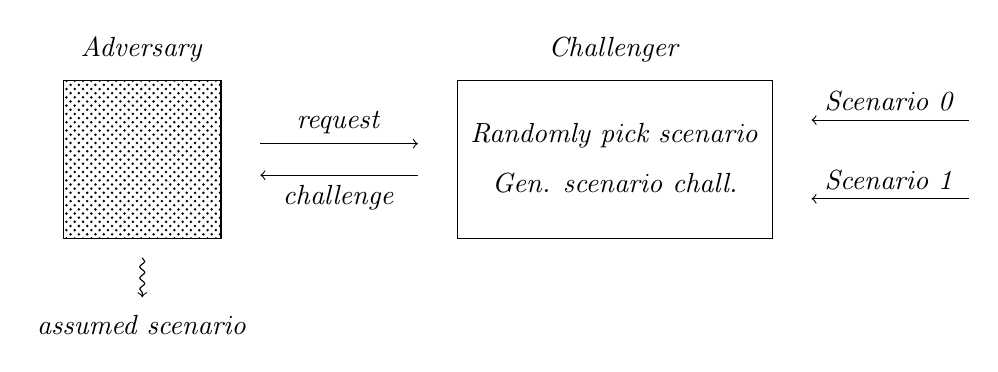
\begin{tikzpicture}[
      Squiggly/.style={
        decorate,
        decoration={snake, segment length=4, amplitude=0.9},
      },
      ]
      \draw[pattern=crosshatch dots] (0, 0) rectangle ++(2,-2);
      \draw (5, 0) rectangle ++(4,-2);
    
      \node (P) at (1, 0.4) {\textit{Adversary}};
      \node (K) at (7, 0.4) {\textit{Challenger}};

      \node[align=center] at (7, -0.7) {\textit{Randomly pick scenario}};
      \node[align=center] at (7, -1.3) {\textit{Gen. scenario chall.}};

      \draw[<-] (9.5, -0.5) -- (11.5, -0.5) node[midway,above] {\textit{Scenario 0}};
      \draw[<-] (9.5, -1.5) -- (11.5, -1.5) node[midway,above] {\textit{Scenario 1}};
    
      \draw[->] (2.5, -0.8) -- (4.5, -0.8) node[midway,above] {\textit{request}};
      \draw[<-] (2.5, -1.2) -- (4.5, -1.2) node[midway,below] {\textit{challenge}};
    
      \draw[->] (1,-2.25) decorate[Squiggly]{ -- (1, -2.75) };
    
      \node (sk) at (1, -3.1) {\textit{assumed scenario}};
    \end{tikzpicture}
    \caption{The flow of a distinguishing game.}
    \label{fig:distinguishing}
  \end{figure}

  \textit{Task.}
  Your task is to implement the distinguishing game between \texttt{strong\_rng()} and \texttt{weak\_rng()} and win it with advantage $\ge 0.8$.
  The following steps outline how to approach this:
  \begin{enumerate}
    \item Implement the challenger:
    \begin{itemize}
      \item Get the challenge size $n$ (in bytes) from the distinguisher.
      \item Randomly sample $n$ bytes of data from either the weak or strong RNG.
      \item Return the data to the challenger.
      \item Return the correct answer (whether it used the weak or strong RNG) to the verifier.
    \end{itemize}
    
    \item Implement the distinguisher:
    \begin{itemize}
      \item Query the challenger for $n$ bytes of challenge,
      \item Process the challenge and try to determine whether the challenger used the weak or strong RNG.
      \item Output the answer to the verifier.
    \end{itemize}

    \item Implement the verifier:
    \begin{itemize}
      \item Ask the distinguisher to run the game many times (e.g. 10).
      \item For each run, get the answer of the distinguisher and of the challenger.
      \item Compute the advantage (the success rate) of the distinguisher.
    \end{itemize}
  \end{enumerate}

  Clearly, if your distinguisher can correctly guess eight out of ten times which of the two generators was used, it has a significant advantage.

  Files: \texttt{lib02.py}, \texttt{leaky\_template.py}
\end{task}

\begin{task}{Learning to dance}
  \textit{Preface}
  ChaCha20 is a widely used pure stream cipher.
  Notably, it is part of the TLS 1.3 recommended ciphers.
  ChaCha20 uses a 256-bit key and a 128-bit \emph{nonce} so that the key can be re-used for encrypting multiple messages.

  The nonce situation is a bit tricky: the \enquote{full nonce} is actually comprised of a little-endian counter, and the \enquote{pure} nonce.
  DJB's \href{https://cr.yp.to/chacha/chacha-20080128.pdf}{\textit{original ChaCha20 proposal}} considers a 64-bit counter and 64-bit nonce.
  This is also what the implementations by \href{https://docs.openssl.org/3.1/man3/EVP_chacha20/#description}{\textit{OpenSSL}} and \href{https://cryptography.io/en/stable/hazmat/primitives/symmetric-encryption/#cryptography.hazmat.primitives.ciphers.algorithms.ChaCha20}{\textit{pyca/cryptography}} use.

  ChaCha20 has also been standardised in \href{https://datatracker.ietf.org/doc/html/rfc8439#section-2.4}{\textit{RFC8439}} and the now obsoleted \href{https://datatracker.ietf.org/doc/html/rfc7539#section-2.4}{\textit{RFC7539}}, where it uses a 32-bit counter and 96-bit nonce.

  \textit{Task.}
  Write a python program that uses pyca/cryptography's \href{https://cryptography.io/en/stable/hazmat/primitives/symmetric-encryption/#cryptography.hazmat.primitives.ciphers.algorithms.ChaCha20}{\texttt{ChaCha20}} class to encrypt a file.
  Then, use OpenSSL's \href{https://docs.openssl.org/master/man1/openssl-enc/}{\texttt{enc}} tool to decrypt it.

  \begin{tcolorbox}[title=Warning]
    While the nonce is not secret and you can safely provide it directly on the command line, you should not provide the key directly on the CLI, as it will stay in your terminal history.
    Instead, you could read it e.g. from a file \texttt{-K "\$(cat key.hex)"}.
    \tcblower
    This is not ideal either because the key is still directly provided as an argument and it might thus leak to other users or processes.
    Unfortunately, the \texttt{enc} tool does not allow providing an alternative key source directly.
    It only provides this capability for the \texttt{-pass} option, where the password can be stored in a file, and the key will be derived from the password.
    Key derivation is a future topic.
  \end{tcolorbox}
\end{task}

\begin{challenge}{Playing the cryptanalyst}
  \textit{Preface.}
  Most programming languages offer some function(s) for generating pseudo-random numbers as part of their standard library.
  Good documentation should always mention whether a method is suitable for producing (pseudo-)randomness of cryptographic quality.
  The rule of thumb is: if the documentation does not mention cryptographic use cases, assume that it is not suitable for cryptographic purposes.

  For Python3, the \texttt{random}\footnotemark{} module can be used to generate \enquote{general purpose} random data, e.g. \texttt{random.randbytes()}.
  \footnotetext{\url{https://docs.python.org/3/library/random.html}}%
  The PRNG uses the \emph{Mersenne-Twister} construction\footnotemark{} (MT), which is a widely used non-cryptographic PRNG due to great statistical properties.
  For example, PractRand will need to parse over 100GB of 32-bit MT data before tests completely fail.
  Still, clever specialised attacks exist against MT making it unsuitable for cryptographic use.%
  \footnotetext{\url{https://en.wikipedia.org/wiki/Mersenne_Twister}}
  
  Most modern programming languages also provide methods for obtaining cryptographically secure pseudo-random numbers.
  Any such functionality must be clearly labelled as such, and even then you should do your research and take the claims with a grain of salt.
  For Python3, cryptographically strong random numbers can be generated with the \texttt{secrets}\footnotemark{} module, e.g. with the \texttt{secrets.token\_bytes()} function.%
  \footnotetext{\url{https://docs.python.org/3/library/secrets.html}}
  Always read the documentation before using functions for cryptography!

  \textit{Task.}
  Implement the distinguishing game between \texttt{secrets.token\_bytes()} (CSPRNG) and \texttt{random.randbytes()} (\enquote{regular} PRNG) and win it with advantage $\ge 0.8$.

  The file \texttt{mtattack.py} contains the \texttt{recover()} function which, if called correctly, will recover the PRNG from the challenge if it was generated with the Mersenne Twister.
\end{challenge}
\end{document}
